\chapter{Differentially Private Multi-Party Communication}
In \Cref{ch:dp-shaping}, we explained our differentially private traffic shaping mechanism. 
In this setup, each end-point only communicates with one other end-point at a time. 
Hence, we excluded e-anonymization attacks, which involve adversaries attempting to uncover the fact that two parties are engaged in communication, rather than revealing the content of the communication.
Furthermore, we assumed a one-hop communication in which the adversary monitors the traffic between two middleboxes.
In order to generalize our findings to scenarios involving multi-party communication, we establish two fundamental communication scenarios: 1- One-to-many communication, and 2- Multi-hop communication. 
We illustrate how we can extend DP guarantees to cover these two scenarios.
Subsequently, we demonstrate that these two communication scenarios adequately serve as building blocks for constructing any arbitrary communication pattern.

\section{One-to-Many Differentially Private Communication}
We assume an application is communicating with $N$ parties at a time.
We extend the notation proposed in \Cref{sec:dp-shaping-definitions} and represent an application stream as a series of $N$ packet sequences:
\begin{equation}
  \istream = <\istream^1, \istream^2, \dots, \istream^N>
\end{equation}
\noindent
where we have:
\begin{align*}
  \istream^1 &= \{{P^{S^1}_1}, {P^{S^1}_2}, {P^{S^1}_3}, \dots \} \\
  \istream^2 &= \{{P^{S^2}_1}, {P^{S^2}_2}, {P^{S^2}_3}, \dots \} \\
  \vdots& \\
  \istream^N &= \{{P^{S^N}_1}, {P^{S^N}_2}, {P^{S^N}_3}, \dots \} 
\end{align*}
\noindent
where $P^{S^k}_i = (l_i^{S^k}, t_i^{S^k})$ indicates that the $i$\textsuperscript{th} input packet sent to $k$\textsuperscript{th} receiving party in communication has length $l_i$ and transmitted at time $t_i$.
\\
\noindent
We make the assumption that all receiving parties are situated behind distinct middleboxes, thereby leading to $N$ parallel communications. \Cref{fig:one-to-many-communication} visually represents this scenario.
This assumption does not restrict the expendability of this scenario as if more than one receiving parties are placed behind the same middlebox, we can merge their packet sequences into one sequence and reduce the number of parallel communications to $N' < N$.   
\begin{figure}[t]
  \centering
  %  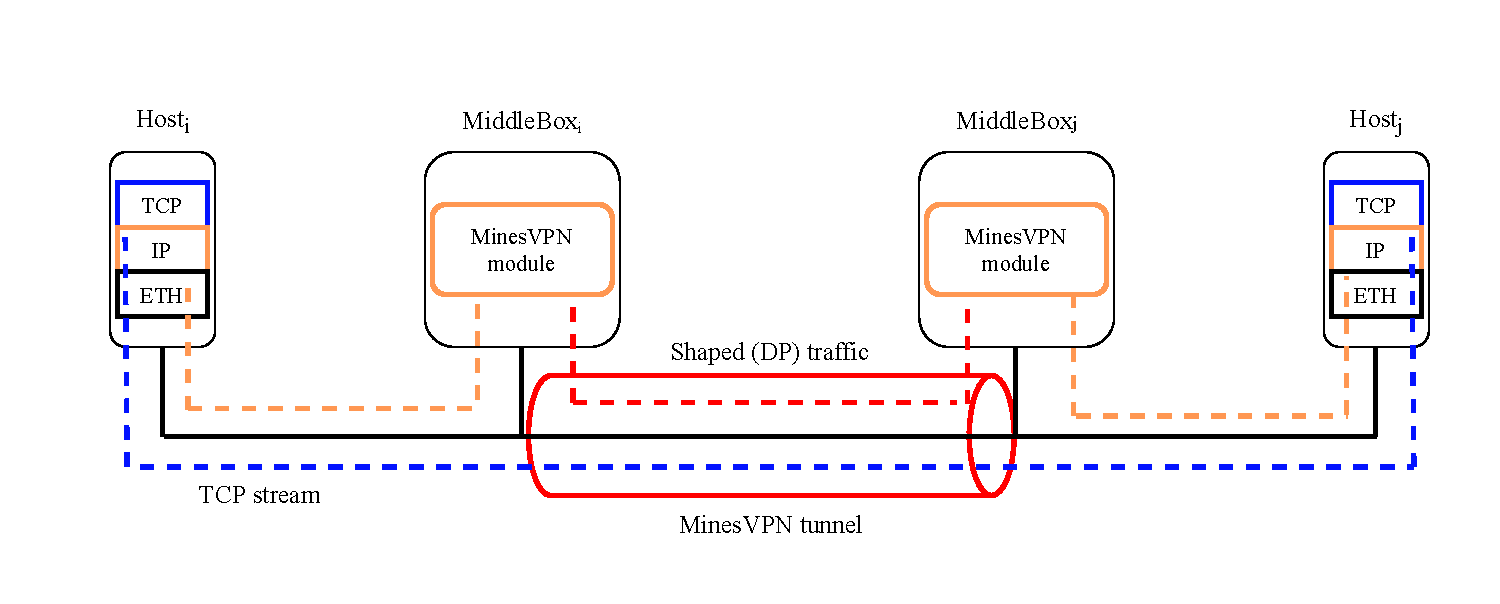
\includegraphics[width=\columnwidth]{figures/Design_highlevel.pdf}
  %  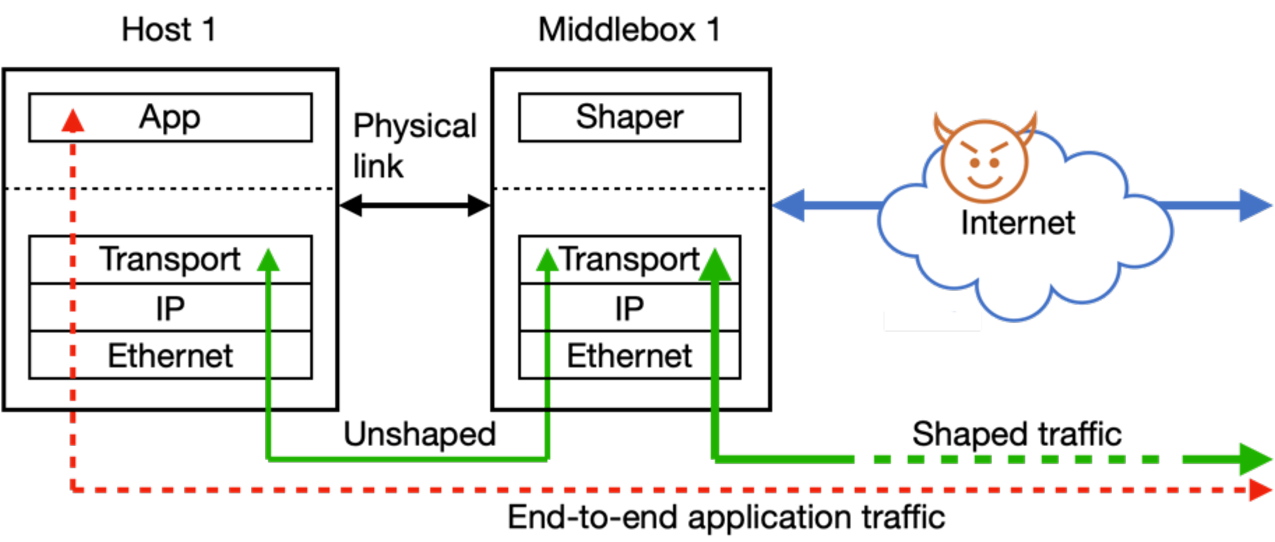
\includegraphics[width=\columnwidth]{figures/minesvpn-overview-half.pdf}
  %  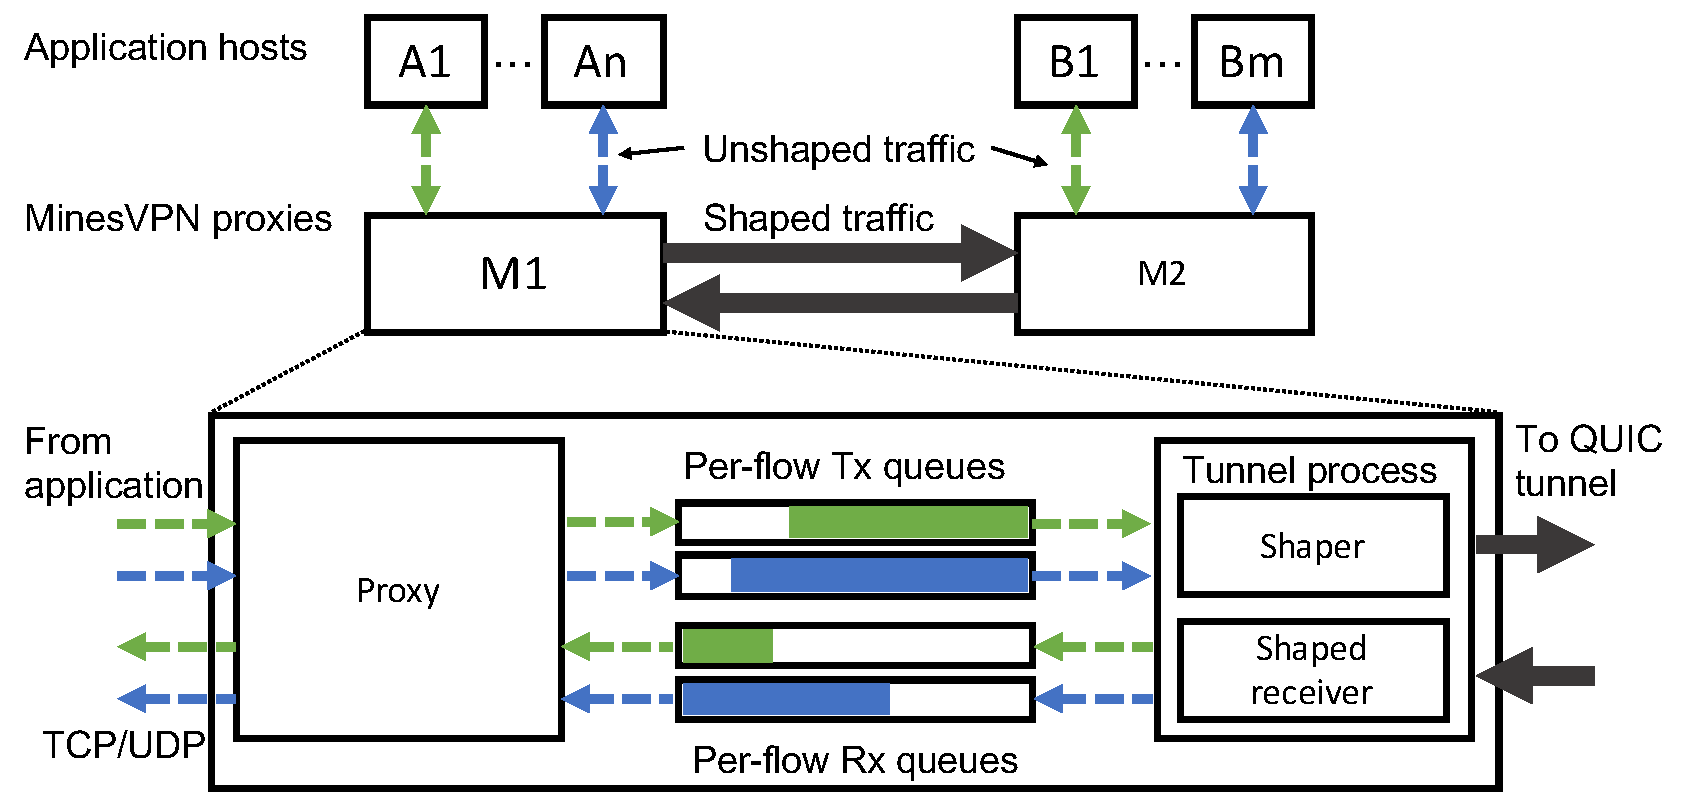
\includegraphics[width=\columnwidth]{figures/minesvpn-arch4.pdf}
  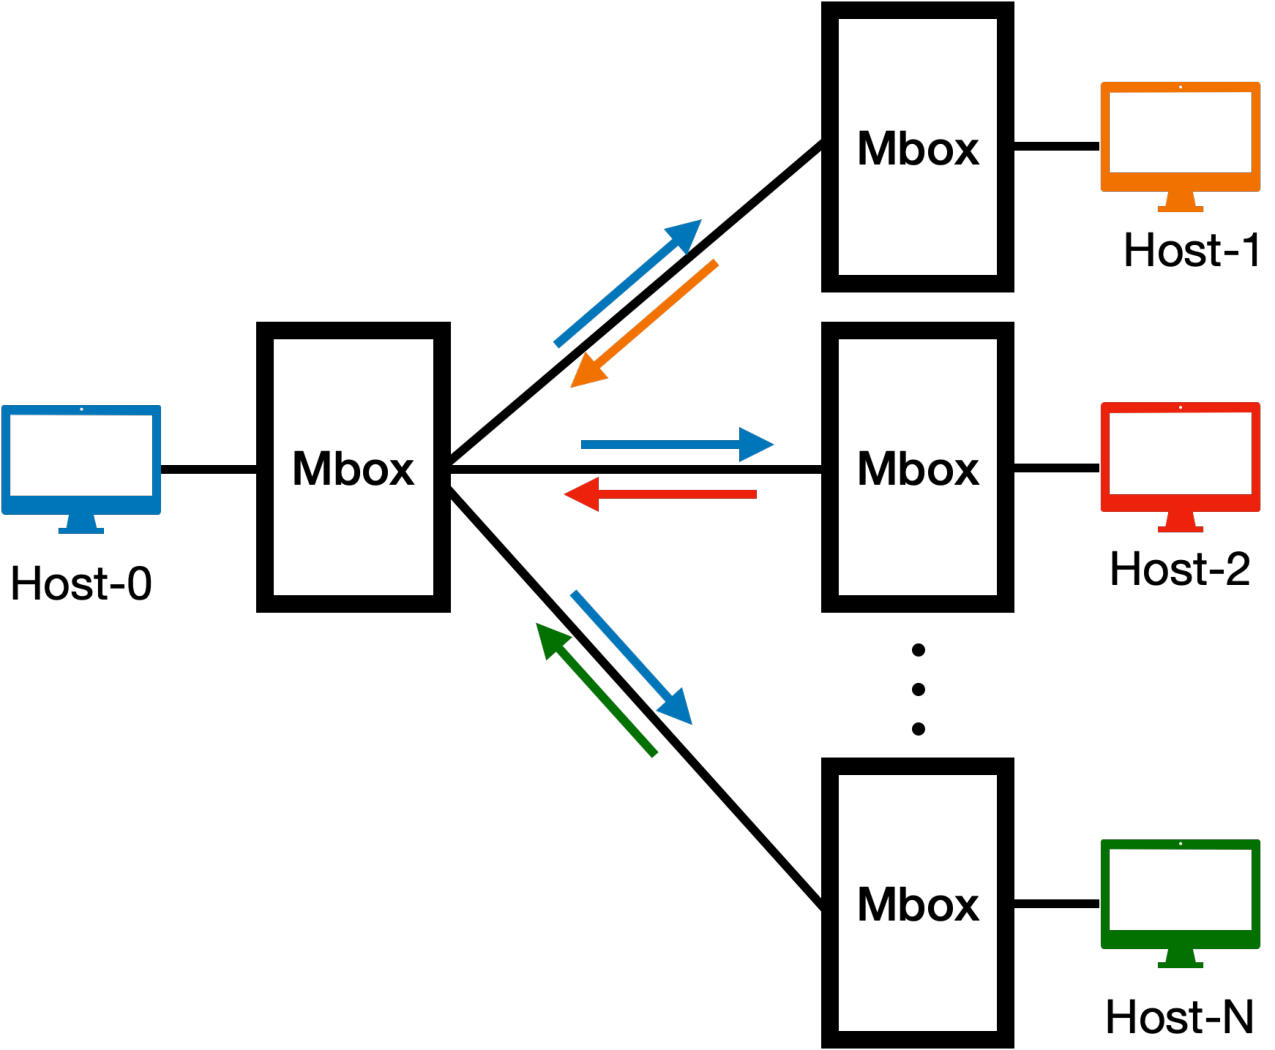
\includegraphics[width=0.7\columnwidth]{figures/one-to-many-communication.pdf}
  \caption{
    One-to-Many parallel communication.
  }
  \label{fig:one-to-many-communication}
\end{figure}



We extend the concept of \textit{buffering queue} that we introduce in \Cref{sec:dp-shaping-definitions} to a \textit{set of $N$ buffering queues} for an application, one for each of pair of communicating parties.  
Each of these queues enqueue the incoming data from application parallel streams with one party within windows of the size of $W$. 
In other words, \Cref{assumption:window} holds true for all $N$ queues simultaneously. 
Similar to \Cref{sec:dp-shaping-definitions}, we define a set of stream subsequences over a window $j$ and represent it with $\istream_j = <\istream^1_j, \istream^2_j, \dots, \istream^N_j>$, such that $k \in [N]:~\istream_j^k = \{P^{\istream^k}_i | P^{\istream^k}_i \in \istream^k~and~t_i^{S^k} \in j\}$. 
Intuitively, a set of stream subsequences is a slice with a length $W$ across all parallel communications with $N$ parties.
We re-define the \Cref{def:neighboring-streams} to match the new setup.
\begin{definition}[Neighboring Series of Streams]\label{def:neighboring-series-stream}
  Two sets of $N$ stream subsequences $S_{j}$ and $\hat{S}_{j}$ transmitted in a window $j$ are neighbors if the L1-norm distance between all corresponding subsequences is at most~$\ssens$ bytes in a window of up to length $\winlen$.
  \\
  In other words: 
  \begin{equation*}
    \forall k \in [n]: {\norm{~S_{j}^k - \hat{S}_{j}^k~}}_1 \leq \ssens
  \end{equation*}
\end{definition}
\noindent
For each subsequence, we define the sensitivity value of its dedicated queue over the intervals of length $T$. 
We represent the sensitivity of a subsequence $S_{j}^k$ with $\qsens^k$: 
\begin{equation}
  \qsens^k = \max_{l = 0}^{\numupdates}~\max_{\streamw{j}^k,
      \hat{\streamw{j}^k}} | \qlent{l}^k - \hat{\qlent{l}^k} |
  \label{eqn:ssens-multi-stream}
\end{equation}
where $\qlent{l}^k$ and  $\hat{\qlent{l}^k}$ are queue lengths of the subsequence $S_{j}^k$ and subsequence $\hat{S_{j}^k}$ at the beginning of the $l$\textsuperscript{th} interval respectively.
The shaping mechanism is independently applied to each packet subsequence, $S_{j}^k$, at intervals of $T$ based on its sensitivity, $\qsens^k$, as we explained in \Cref{subsec:dp-shaping-mechanism}.
Therefore, each queue measurement is $(\varepsilon_T, \delta_T)$-DP.
The transmitted packet sequence is denoted as $N$ sequences of packets observable by adversary:
\begin{equation}
  \ostream = <\ostream^1, \ostream^2, \dots, \ostream^N>
\end{equation}
\noindent 
where we have:
\begin{align*}
  \ostream^1 &= \{{P^{O^1}_1}, {P^{O^1}_2}, {P^{O^1}_3}, \dots \} \\
  \ostream^2 &= \{{P^{O^2}_1}, {P^{O^2}_2}, {P^{O^2}_3}, \dots \} \\
  \vdots& \\
  \ostream^N &= \{{P^{O^N}_1}, {P^{O^N}_2}, {P^{O^N}_3}, \dots \} 
\end{align*} 
We assume that the adversary's goal is to expose the contents of a single packet sequence, $\ostream^k$.
In pursuit of this objective, the adversary strategically exploits the information made available through other packet sequences.
To calculate the privacy loss of measuring all queues for all stream subsequences at each interval, we need to differentiate between two different communication setup: Independent subsequences and Correlated subsequences.   

To measure dependency between stream subsequence, we use the correlation between two streams such that for an application stream with $N$ series of packet sequences $\istream = <\istream^1, \istream^2, \dots, \istream^N>$, we have:
\begin{equation*}
  \forall i,j \in [N]:~Corr(\istream^i, \istream^j) = c_{ij}
\end{equation*}
\noindent
This enables us to define a correlation matrix $C$ such that $[C]_{ij}=c_{ij}$.
We assume the correlation coefficients to have the following properties:
\begin{enumerate}
  \item For all $i,j \in [N]$, $-1 \leq c_{ij} \leq 1$, with $-1$ representing that two subsequences are negatively correlated (\ie when one exists in the stream the other one does not and vice versa), $1$ representing that they are fully correlated (\ie they appear in the stream always together), and $0$ means no correlation.
  \item For all $i \in [N]$, $c_{ii} = 1$.
\end{enumerate}
Various correlation metrics fulfill the aforementioned conditions, with the Pearson correlation coefficient~\cite{cohen2009pearson} being the most prevalent among them. 
\noindent
Calculating privacy loss for independent sequences (\ie $\forall i \neq j \in [N]:~corr(\istream^i, \istream^j) = 0$) is straightforward. 
In independent communication setup, monitoring one sequence does not reveal any information about others. 
Therefore, each stream subsequence is $(\varepsilon_T, \delta_T)$-differentially private.
Nonetheless, in a correlated setup, the adversary has the ability to monitor a single stream, thereby acquiring preceding information about others, which consequently results in further privacy breaches. 
In the following section, we present a systematic approach for quantifying privacy loss in interdependent stream subsequences.
















% \subsection{One-to-Many Independent Communication}
% In this regime of communication, We assume an application is communicating with $N$ parties independently.
% If we represent an application stream with $N$ series of packet sequences $\istream = <\istream^1, \istream^2, \dots, \istream^N>$, all packet sequences are mutually uncorrelated:
% \begin{equation*}
%   \forall i \neq j \in [N]:~corr(\istream^i, \istream^j) = 0
% \end{equation*}
% \noindent
% This assumption is particularly correct for message passing and video streaming applications as these applications provide service for non-related entities.
% For this setup, we argue that the privacy loss of measuring all subsequence queues with DP is the same as privacy loss associated with each individual queue.
% \begin{proposition}\label{prop:independent-subsequence}
%   Assume all packet sequences within an application stream are mutually uncorrelated, if we measure each subsequence queue size with $(\varepsilon_T, \delta_T)$-DP with a sensitivity of $\qsens^k$, measuring queue sizes for all subsequences is also $(\varepsilon_T, \delta_T)$-DP.  
% \end{proposition} 
% \begin{proof}
%   (informal) As packet subsequences are independent, releasing a DP measurement of a queue for one subsequence does not affect the adversary's prior knowledge regarding any other subsequences. 
%   Therefore, the privacy loss associated with the communication between a single pair does not change. 
% \end{proof}
% \noindent
% Based on \Cref{prop:independent-subsequence}, we can measure the privacy loss of a 1-to-$N$ communication simply by extending results of \Cref{prop:dp} to a multiparty communication as follows:
% \begin{proposition}\label{prop:independent-stream-privacy}
%   In the one-to-many independent communication setup, {$\sys$} enforces $(\varepsilon_{\winlen}, \delta_{\winlen})$-DP for each pair of communicating entities within the window of length $W$, with $\varepsilon_{\winlen}, \delta_{\winlen} \triangleq
%   \textrm{DP\_compose}(\varepsilon_T, \delta_T, \numupdates)$.
% \end{proposition}


\subsection{One-to-Many Correlated Communication}
In many applications,  simultaneous communications with distinct entities are interdependent.
For example, many businesses use online advertising platforms such as Google Ads to create and run ads on various websites.
Therefore, every time a user requests the website, the web browser retrieves content from both the web server hosting the website and the online advertising platform that hosts the website's Ads.   
This is, in fact, an example of a one-to-many correlated communication setup.
\\
In standard definition of differential privacy, we assume data points to be independent.  
However, measuring the privacy loss when entries of database are correlated is challenging.
We use two different approaches to tackle this problem. 
\subsubsection{Adjusting Sensitivity for Correlated Communication}


\subsubsection{Composition of Privacy Loss for Correlated Communication}


One approach to ensure DP guarantees for a correlated communication involves multiplying the sensitivity of each packet sequence by the number of correlated packet sequences (\ie $((\qsens^k)_{corr}) = N.\qsens^k$).
Chen\etalc{chen2014correlated} prove this approach to be differentially private.
However, this method implicitly assumes that all correlated sequences are fully correlated, leading to excessive overhead.
To avoid this assumption, we use correlated differential privacy setup proposed by Zhu\etalc{zhu2014correlated} to calculate the privacy loss of our shaping mechanism in one-to-many correlated communication regime.

Following the approach of Zhu~\etal, for each packet sequence, we define correlated sensitivity for each packet sequence:
\begin{definition}[Correlated Sensitivity]\label{def:correlated-sensitivity} 
  For each packet subsequence $S_{j}^k$, we define the correlated sensitivity value of its dedicated queue over the interval of length of $T$, and calculate it as follows:
  \begin{equation}\label{equ:correlated-sensitivity}
    (\qsens^k)_{corr} = \sum_{m=0}^{N} |c_{mi}|. \big( \max_{l = 0}^{\numupdates}~\max_{\streamw{j}^m,
    \hat{\streamw{j}^m}} | \qlent{l}^k - \hat{\qlent{l}^k} | \big) 
  \end{equation}
\end{definition}
\noindent Intuitively, the correlated sensitivity for a packet sequence captures the effect of adding/removing all other packet sequences on the designated sequence.
From \Cref{def:correlated-sensitivity}, it is clear that:
\begin{equation*}
  \qsens^k \leq (\qsens^k)_{corr} \leq N.\qsens^k
\end{equation*} 
\noindent
With \Cref{def:correlated-sensitivity}, we can re-state \Cref{prop:independent-subsequence} for correlated packet sequences.
\begin{proposition}\label{prop:dependent-subsequence}
  Assume there is correlation between packet subsequences of an application stream, if we measure each subsequence queue size with $(\varepsilon_T, \delta_T)$-DP with a sensitivity of $(\qsens^k)_{corr}$ (see \ref{equ:correlated-sensitivity}), measuring queue sizes for all subsequences is also $(\varepsilon_T, \delta_T)$-DP.  
\end{proposition}
\begin{proof}
  Zhu\etalc{zhu2014correlated} prove that if we scale the noise of a randomized differentially private randomized mechanism with adjusted the sensitivity of \Cref{equ:correlated-sensitivity}, it provides DP. The privacy of our mechanism naturally derives from this statement. 
\end{proof}
\noindent Similarly, \Cref{prop:independent-stream-privacy} holds true for interdependent packet sequences within an application stream. 
\begin{proposition}\label{prop:dependent-stream-privacy}
  In the one-to-many correlated communication setup, {$\sys$} enforces $(\varepsilon_{\winlen}, \delta_{\winlen})$-DP for each pair of communicating entities within the window of length $W$, with $\varepsilon_{\winlen}, \delta_{\winlen} \triangleq
  \textrm{DP\_compose}(\varepsilon_T, \delta_T, \numupdates)$.
\end{proposition}

